\ifnotes
\else
  \PassOptionsToClass{handout}{beamer}
\fi

\documentclass[10pt,t]{beamer}

\usetheme{metropolis} % use metropolis theme

\usepackage{solarized}            % use solarized themed listings
\usepackage{appendixnumberbeamer} % do not number appendix frames
\usepackage[scale=3]{ccicons}     % creative commons icons

% fix-up the handling of the notes pages
\ifnotes
  \hypersetup{final}
  \usepackage{pgfpages}
  \setbeamertemplate{note page}[plain]
  \setbeameroption{show notes on second screen=right}
\fi

%-------------------------------------------------------------------------------

\usepackage{tabularx}
\usepackage{tikz}
\usetikzlibrary{decorations.pathreplacing}

\title{Introduction to Cuda}
\date{}
\author{Jeremy Iverson}
\institute{College of Saint Benedict \& Saint John's University}
\begin{document}
  \maketitle

  \begin{frame}{execution model}
    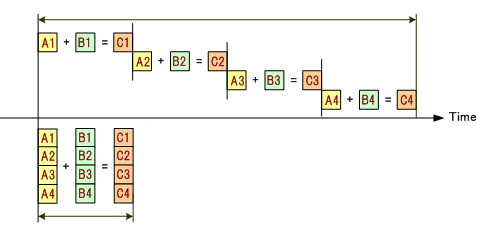
\includegraphics[width=\textwidth]{simd-execution.png}\\
  \end{frame}

  \begin{frame}{gpu architecture}
    \only<1>{\includegraphics[width=.70\textwidth]{k210-die.png}}
    \only<2>{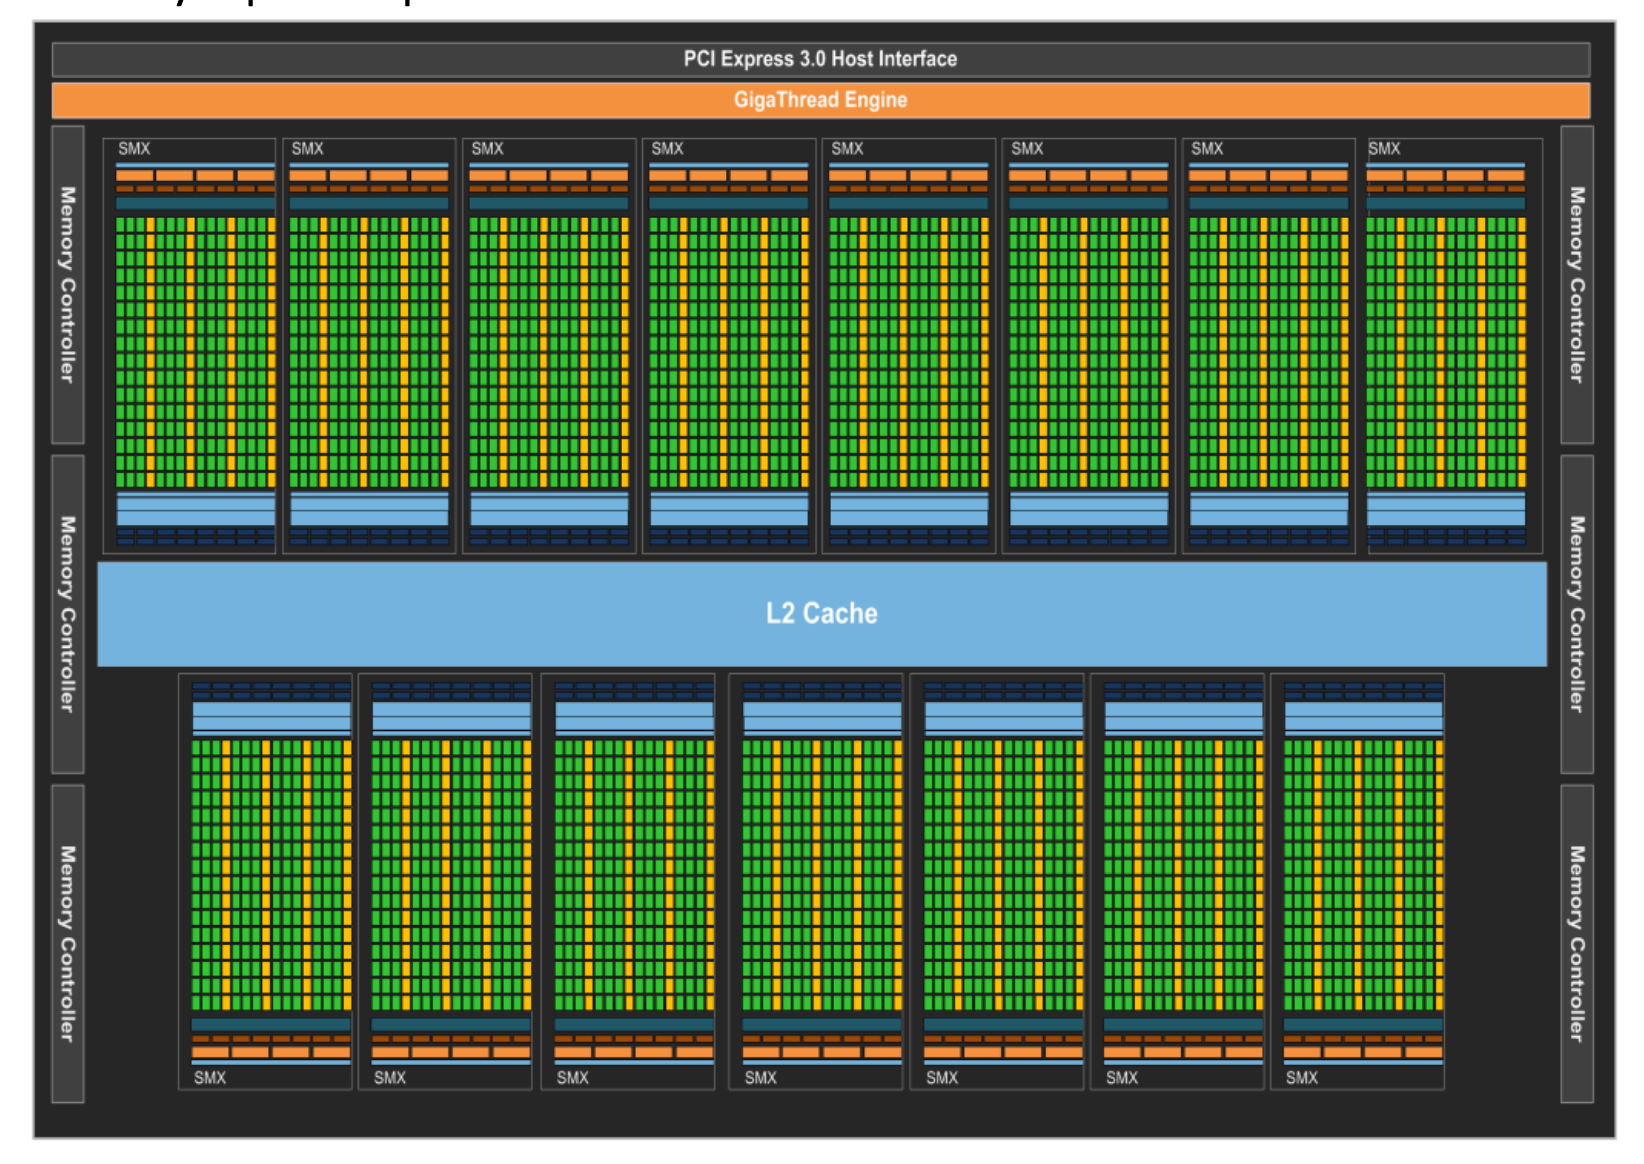
\includegraphics[width=\textwidth]{k210-arch.png}}
  \end{frame}

  \begin{frame}{k210 streaming multiprocessor (SMX)}
    \hspace{-25ex}
    \begin{columns}[T]
      \begin{column}{.56\textwidth}
        \begin{itemize}
          \item 13 SMX per device
            \begin{itemize}
              \item 192 SP CUDA cores
              \item 64 DP CUDA cores
              \item 128KB shared memory / L1 cache
              \item 48KB read-only data cache
              \item 128K 32-bit registers
            \end{itemize}
          \item 1536KB L2 cache (shared)
          \item 12GB DRAM
          \item 562MHz base w/ 824MHz boost
          \item<2> Theoretical 4.113TFLOP/s
        \end{itemize}
      \end{column}
      \begin{column}{.51575\textwidth}
        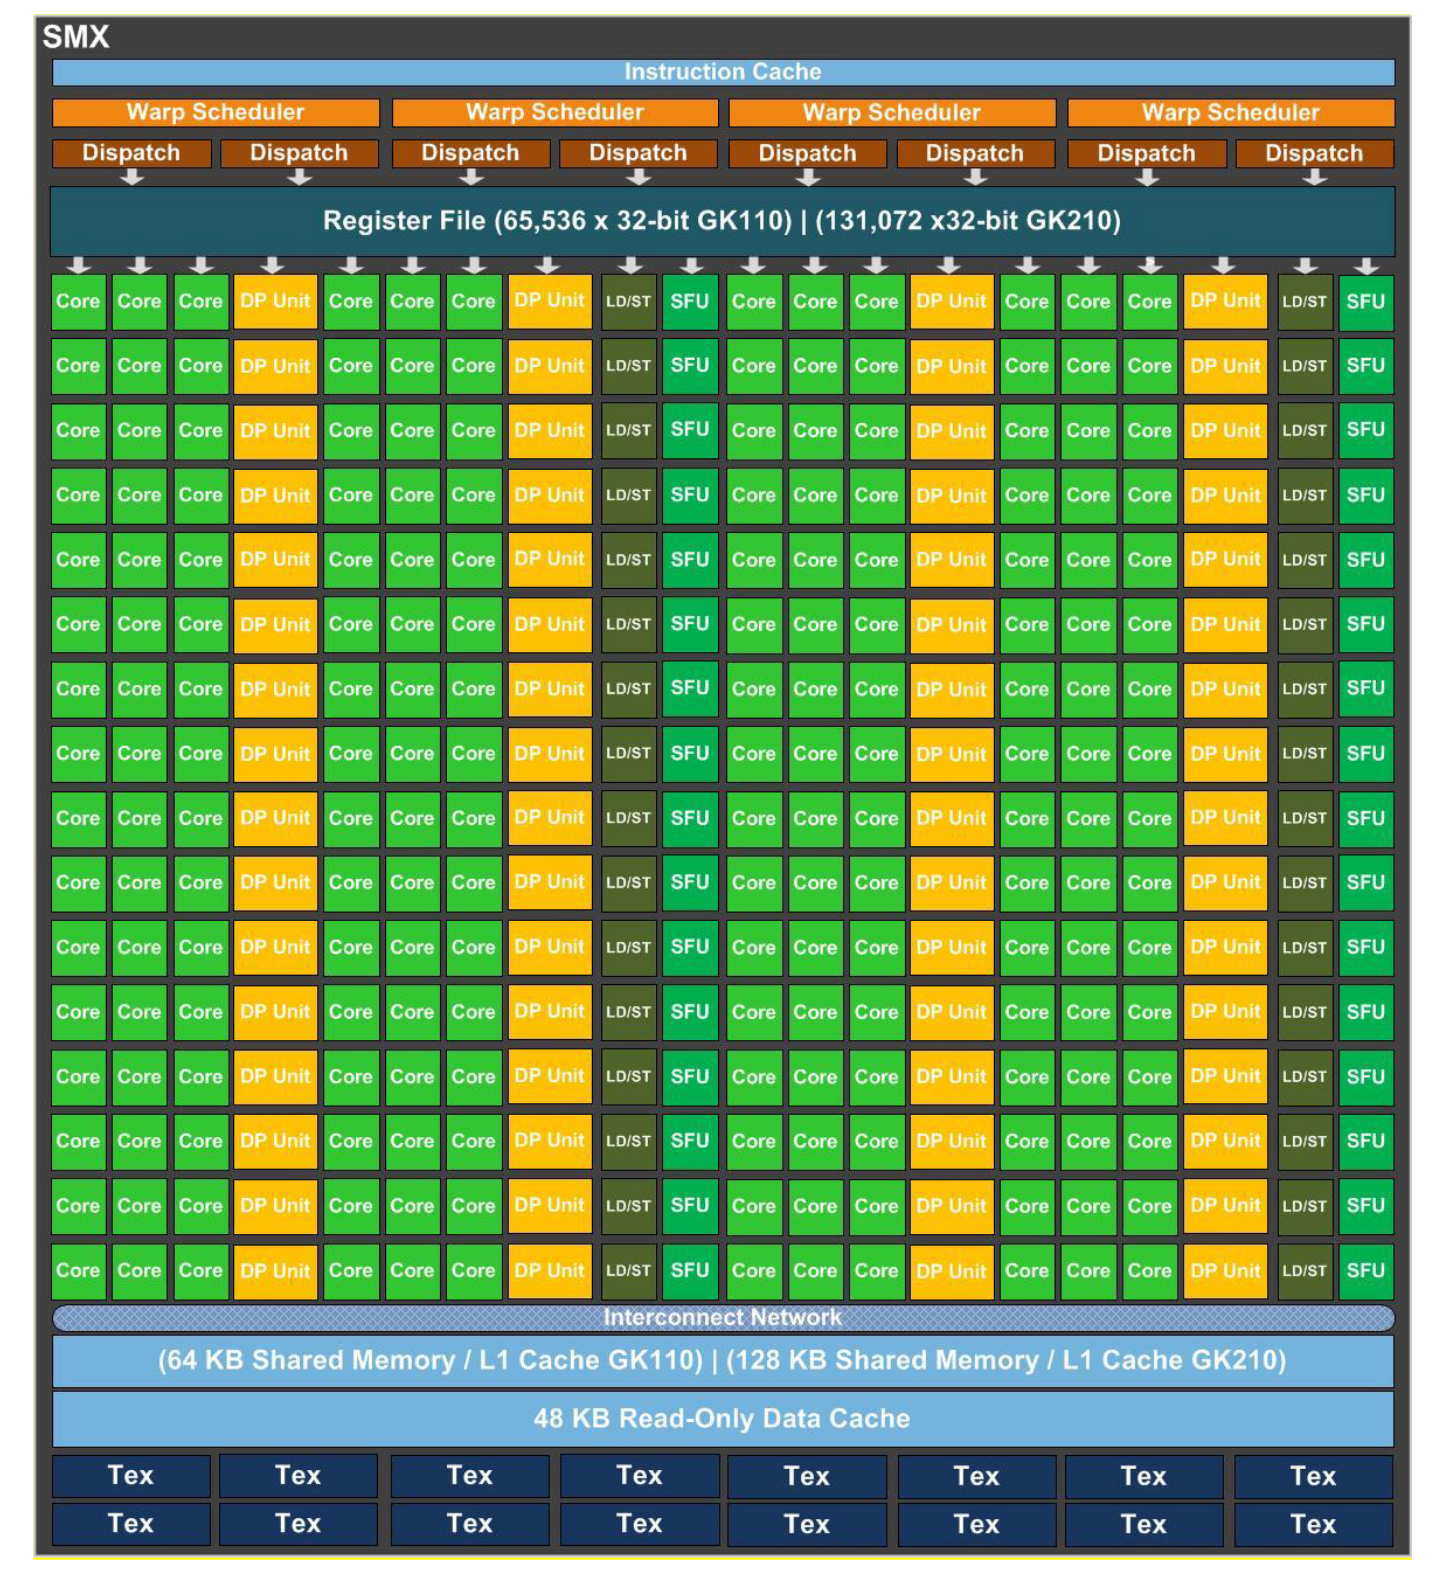
\includegraphics[width=\textwidth]{k210-smx.png}
      \end{column}
    \end{columns}

    \note[item] { $824,000,000 \times 2496 \times 2 = 4,113,408,000,000 =
    4.113$TFlop/s -- the final $\times 2$ is because the GPU can issue a
    floating-point multiply and floating-point add as a single instruction
    (fused-multiply-add), so one instruction counting as two operations. }
  \end{frame}

  \begin{frame}{gpu execution model}
    \begin{itemize}
      \item SIMT (single-instruction multiple-thread)
      \item SMX executes threads in groups of 32 threads, called warps
        \begin{itemize}
          \item two independent instructions per warp can be issued per cycle
        \end{itemize}
      \item warps are organized into blocks
        \begin{itemize}
          \item a set of concurrently executing threads that can cooperate
            through synchronization and shared memory
        \end{itemize}
      \item hardware multi-threading (as opposed to OS)
        \begin{itemize}
          \item context switching is basically free
        \end{itemize}
    \end{itemize}

    \note[item] {a result of dual issue is that 16 threads will be executing
      the same instruction... always}
    \note[item] {hardware multi-threading as opposed to OS, i.e., logic is
      built into card to support multi-threading, makes context switching
      basically free}
  \end{frame}

  \begin{frame}{memory scopes}
    \begin{itemize}
      \item per thread private memory (allocated in register file)
      \item per block shared memory (allocated in shared memory)
        \begin{itemize}
          \item threads in different blocks cannot access each others per block
            shared memory
        \end{itemize}
      \item global memory (allocated in DRAM)
        \begin{itemize}
          \item can be accessed by any thread, any time
        \end{itemize}
    \end{itemize}
  \end{frame}

  \begin{frame}[standout]{}
    \centering
    CUDA
  \end{frame}

  \begin{frame}{CUDA programming}
    \begin{itemize}
      \item Program GPU to complement CPU
      \item Augment C/C++ with minimalist abstractions
      \item Provide straightforward mapping onto hardware
        \begin{itemize}
          \item good fit to GPU architecture
          \item maps well to multi-core CPUs too
        \end{itemize}
      \item Scale to 1000s of parallel threads
        \begin{itemize}
          \item gpu cores are lightweight (create / switch is free)
          \item gpu uses 1000s of threads to hide latency
        \end{itemize}
    \end{itemize}
  \end{frame}

  \begin{frame}{CUDA parallelism model}
    \begin{itemize}
      \item a parallel computation is initiated by executing a kernel function
        from the host (CPU)
        \begin{itemize}
          \item kernel function runs to completion and returns control back to
            the host
        \end{itemize}
      \item parallel threads are organized in a two-level hierarchy: threads and
        blocks
        \begin{itemize}
          \item a computation contains a set of blocks, each block containing
            the same number of threads
          \item threads in a block can communicate and synchronize
          \item in general, threads in different blocks cannot synchronize
        \end{itemize}
    \end{itemize}
  \end{frame}

  \begin{frame}{CUDA parallelism model cont'd}
    \begin{itemize}
      \item blocks themselves are organized into a 3D grid -- this is for
        convenience to the programmer -- it can help map blocks to the parts of
        a problem that they are working
      \item blocks can be scheduled for execution on an SMX in any order
        \begin{itemize}
          \item multiple blocks can be scheduled to the same SMX, as long as
            there are sufficient resources available
          \item once scheduled, a block will run to completion
        \end{itemize}
    \end{itemize}
  \end{frame}

  \begin{frame}{C for CUDA}
    \begin{itemize}
      \item Function qualifiers:
        \begin{itemize}
          \item \texttt{\_\_global\_\_ void my\_kernel() { }}
          \item \texttt{\_\_device\_\_ float my\_device\_func() { }}
        \end{itemize}

      \item Execution configuration:
        \begin{itemize}
          \item \texttt{dim3 grid\_dim(100, 50); // 5000 thread blocks}
          \item \texttt{dim3 block\_dim(4, 8, 8); // 256 threads per block}
          \item \texttt{my\_kernel<<<grid\_dim,block\_dim>>>(...); // Launch}
        \end{itemize}
      \item Built-in variables and functions valid in device code:
        \begin{itemize}
          \item \texttt{dim3 gridDim; // Grid dimension}
          \item \texttt{dim3 blockDim; // Block dimension}
          \item \texttt{dim3 blockIdx; // Block index}
          \item \texttt{dim3 threadIdx; // Thread index}
          \item \texttt{void \_\_syncthreads(); // Thread synchronization}
        \end{itemize}
    \end{itemize}
  \end{frame}

  \begin{frame}[fragile]{vector addition}
    \begin{codeblock}
    __global__ void
    vector_add(float *A, float *B, float *C) {
      int idx = blockIdx.x * blockDim.x + threadIdx.x;
      C[idx] = A[idx] + B[idx];
    }

    int main() {
      // Initialization code
      ...
      // Run N/256 blocks of 256 threads each
      vector_add<<<N/256,256>>>(d_A, d_B, d_C);
    }
    \end{codeblock}
  \end{frame}

  \begin{frame}[fragile]{vector addition cont'd}
    \begin{codeblock}
     // allocate host (CPU) memory
     float *h_A = ..., *h_B = ...;

     // allocate device (GPU) memory
     float *d_A, *d_B, *d_C;
     cudaMalloc( (void**) &d_A, N * sizeof(float));
     cudaMalloc( (void**) &d_B, N * sizeof(float));
     cudaMalloc( (void**) &d_C, N * sizeof(float));

     // populate h_A and h_B
     ...

     // copy host memory to device
     cudaMemcpy(d_A, h_A, N * sizeof(float),
      cudaMemcpyHostToDevice);
     cudaMemcpy(d_B, h_B, N * sizeof(float),
      cudaMemcpyHostToDevice);
    }
    \end{codeblock}
  \end{frame}

  \appendix

  \begin{frame}[c]
    \begin{center}\ccbysa\end{center}

    except where otherwise noted, this worked is licensed under
    \href{http://creativecommons.org/licenses/by-sa/4.0/}{creative commons
    attribution-sharealike 4.0 international license}
  \end{frame}
\end{document}
